%----------------------------------------------------------------------------
%  scoping_state_monad.tex 
%----------------------------------------------------------------------------

Let us now focus on the notion of variable scope that is implicit in a monad. Whenever we bind two statements, the scope of the bound value is limited to the body of the second parameter (unless it is returned). This means that after the bound value is passed to the second parameter, then its lifetime is exhausted and the value may be decremented. Of course, whenever we return a value then to prevent its premature reclamation we will increment it to counter its decrementing by the enclosing binding.
The new type of the bind and return operators now requires that these two only manipulate monads to references. Bind will also decrement the bound value as soon as it goes out of scope:

\begin{lstlisting}
(>>=) :: Reference f a s => St s (f a) -> (f a -> St s b) -> St s b
p >>= k = \s ->
  let y,s' = p s
  let z,s'' = k y s'
  in z,snd(decr y s'')
\end{lstlisting}

while return will increment its parameter:

\begin{lstlisting}
return :: Reference f a s => f a -> St s (f a)
return x = \s -> x,snd(incr x s)
\end{lstlisting}

This is convenient because in the rest of the paper we will have no need to use those as standalone monadic statements and instead we will use them only as functions from state to state.

\subsection{General recursion}

Whenever we are in the presence of stateful recursive functions, then we may find that some embarrassing facts occur. In particular, the lifetime of a local value inside the body of the recursive function may be unnaturally lengthened to encompass the entire sub-trees of the recursive call. This is unacceptable, especially if we think about functions that recursively open a lot of files (like when traversing the file system in search for something) or use a lot of memory.


\subsubsection{Benchmark}

Let us consider a very challenging example of this scenario. We wish to create a balanced binary tree from a set of points:

\begin{lstlisting}
bt :: [Point] -> Tree [Point]
bt pts =
  if size pts < 1000 then mk_leaf pts
  else
    let m = median pts
    let l,r = split pts m
    let tl = bt l
    let tr = bt r
    in mk_node (tl,tr)
\end{lstlisting}

In this example we can clearly see that until both calls to bt l and bt r are completed, then we may not release any memory at all! This is clearly nonsense, since pts can be released right after the call to split and l can be released right after the first recursive call to bt.


\subsubsection{Explicit continuations}

Enter Continuation Returning Style. We try and solve this problem with trampolines \cite{7_7}, that is intermediate pieces of code that are "wrapped" around our recursive calls. We will call this style Continuation Returning Style because statements in this style do not return their result when executed but rather return another statement which, when executed in its turn, will complete the job. We refer to this nested statement as a trampoline. We define trampolines as statements that capture by (explicit) closure a containing Reference which gets incremented when the trampoline is created and which is released after the trampoline is executed.
Using trampolines does not exclude the possibility of using the state monad as defined above. Whenever its conservative notion of lifetime is acceptable, we will be free to use it; whenever its notion of lifetime is too restrictive, then we will use our trampolines and jump between the two easily. A trampoline is defined as:

\begin{lstlisting}
type Trmp s a = St s (St s a)
\end{lstlisting}

It may help understanding trampolines in terms of the following diagram which shows the order in which the state flows:

\begin{figure}[h]
\centerline{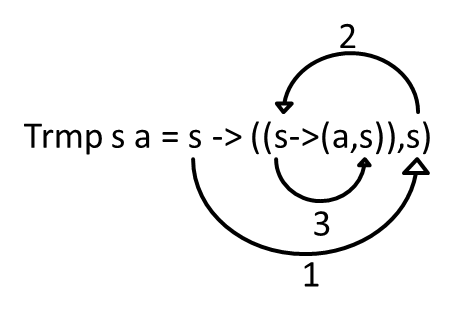
\psfig{file=TrmpDiagram.png,height=5cm}} 
\caption{State flow\label{fig:trampoline_diagram}}
\end{figure}

A trampoline is constructed from the captured values that will have a lifetime at least as long as that of the trampoline and the actual body of the trampoline. The first thing the trampoline constructor does is increment the captured values, and then it binds the execution of the body of the trampoline with decrementing the captured values:

\begin{lstlisting}
trmp :: Reference f a s => f a -> (f a -> Trmp s b) -> Trmp s b
trmp ctxt p = \s -> (\s ->
  let p',s' = p ctxt s
  in p' (snd (decr ctxt s'))), snd (incr ctxt s)
\end{lstlisting}

We have a return function that creates a trampoline. To make this work we assume that our language supports operator overloading, where the most specific overload will be invoked at each binding site:

\begin{lstlisting}
return :: Reference f a s => f a -> Trmp s (f a)
return x = \s->(\s -> x,snd (incr x s)),s
\end{lstlisting}

We can turn a trampoline into a statement with relative ease by unpacking it and executing it twice:

\begin{lstlisting}
(!) :: Trmp s a -> St s a
!p = \s ->
  let p',s' = p s
  in p' s'
\end{lstlisting}

Even more interesting is the fact that we can easily bind values of the state monad with trampolines;  the result will be another trampoline. This kind of binding starts decrementing the bound value y much sooner than the standard binding, since y get decremented before the full execution of k. The idea is that k has a chance to increment y as its ctxt, and right after this has been done k y returns k'. The actual execution of k is thus stored as k', which may contain recursive calls to some caller. Before executing this (possibly time-consuming) code we get our chance to free y in case it were not needed anymore inside k':

\begin{lstlisting}
(>>=) :: Reference f a s => St s (f a) -> (f a -> Trmp s b) -> Trmp s b
p >>= k = \s ->
  let y,s' = p s
  let k',s'' = k y s'
  in k', decr y s''
\end{lstlisting}

Notice that this version of the binding operator is exactly the same as the original binding operator, and since trampolines are state monads then there is no need for the explicit definition.

\subsubsection{Solving the benchmark problem}

We can rewrite the binary tree example above as:

\begin{lstlisting}
bt :: Reference f [Point] s => f [Point] -> Trmp s Tree [Point]
bt pts =
  if size pts < 1000 then trmp pts (\pts -> return mk_leaf pts)
  else
    trmp pts (\pts ->
      do m <- median pts
         trmp (pts,m) (\(pts,m) ->
           do l,r <- split pts m
              trmp (l,r) (\(l,r) -> 
              do tl <- bt l
                 trmp (tl,r) (\(tl,r) ->
                 do tr <- bt r
                    trmp (tl,tr) (\(tl,tr) ->
                      return mk_node (tl,tr))))))
\end{lstlisting}

where we can clearly see that each continuation declares explicitly what it will keep alive (in terms of reference counting). This is a similar style to the well-known world-passing-style of the state monad, but we are also passing around the active scope.

\subsubsection{Syntactic sugar for continuations}

It is very important to notice a detail that threatens the correctness of our system. Continuations may not capture values whose type respects the Reference predicate; continuations may only use those counters that they explicitly captured, otherwise we have no guarantee that the captured counter will still be valid when accessed.
For this reason we introduce a notion of syntactic sugar for expressing our continuations where the captured variables are the free variables of type Reference accessed in the body of the continuation. We tell the compiler to search for these variables with the trmp keyword (not to be confused with the private trmp function seen above).
The translation rule is quite straightforward:

\begin{lstlisting}
	[| trmp x <- m n |] = trmp ctxt (\ctxt -> m >>= fun x -> [| trmp n|])	
	where ctxt = FC(m) $\cup$ FC(n)

	[| trmp return m |] = trmp ctxt (\ctxt -> return m)
	where ctxt = FC(m)
where FC(t) = {x:f a $\in$ FV(t) : $\exists$s . Reference f a s}
\end{lstlisting}

The resulting code is:

\begin{lstlisting}
bt :: Reference f [Point] s => f [Point] -> Trmp s Tree [Point]
bt pts =
  if size pts < 1000 then trmp return mk_leaf pts
  else
    trmp m <- median pts       -- FC = pts
       l,r <- split pts m      -- FC = m,pts
       tl <- bt l              -- FC = l,r
       tr <- bt r              -- FC = r,tl
       return mk_node (tl,tr)  -- FC = tl,tr
\end{lstlisting}

and since we can easily see that:

\begin{lstlisting}
FC(trmp m <- median pts
        l,r <- split pts m 
        tl <- bt l 
        tr <- bt r 
        return mk_node (tl,tr)) = pts
FC(trmp l,r <- split pts m 
        tl <- bt l 
        tr <- bt r 
        return mk_node (tl,tr)) = (pts,m)
FC(trmp tl <- bt l 
        tr <- bt r 
        return mk_node (tl,tr)) = (l,r)
FC(trmp tr <- bt r
        return mk_node (tl,tr)) = (tl,r)
FC(return mk_node (tl,tr)) = (tl,tr)
\end{lstlisting}

then it is clear how the sample with implicit continuations becomes identical to the one with explicit continuations.

